\maketitle
\textbf{Enunciado: } Simule un sistema de filas \textbf{M/M/7/7} con $\lambda=2$ y $\mu=4$. Utilizando la simulación, determine $L_s$ y $T_s$.\vspace{1cm}

\textbf{Resultados\\}
Los valores teóricos se obtuvieron al evaluar las fórmulas estudiadas en clase para las colas \textbf{M/M/7/7}:
\begin{equation}\label{eq:teo}
    \begin{split}
        &\rho = \lambda/\mu\\
        &\pi(0) = \left(\sum_{n=0}^7\dfrac{\rho^n}{n!}\right)^{-1}\\
        &\pi(c)=\dfrac{\rho^7}{7!}\pi(0)\\
        &L_s=\rho(1-\pi(7))\\
        &T_s=L_s/\lambda
    \end{split}
\end{equation}
y se llegó a $L_s\approx0.5$ y $T_s\approx0.25$.
La simulación fue realizada utilizando el paquete \texttt{simmer} \cite{simmer} en R. La implementación está basada en los ejemplos mostrados en \cite{ex_simmer} y \cite{ex_simmer2}.

A continuación se explicará, sin mucho detalle, el código implementado.

\begin{enumerate}
    \item Importar los paquetes e inicializar una semilla para la simulación (se utilizó la misma de los ejemplos): 
        \begin{lstlisting}
        library(simmer)
        library(simmer.plot)
        set.seed(1234)
        \end{lstlisting}
    \item Inicialización de los parámetros de la simulación: $\lambda$, $\mu$, $c$ y el tiempo de simulación:
        \begin{lstlisting}
        lambda <- 2
        mu <- 4
        c <- 7
        T <- 600
        \end{lstlisting}
    \item Creación de la actividad (su duración) con su respectiva cola:
        \begin{lstlisting}
        m.queue <- trajectory() % >%
            seize('server', amount=1) % >%
            timeout(function() rexp(1, mu)) % >%
            release('server', amount=1)
        \end{lstlisting}
    \item Llegadas al sistema con su capacidad $c$ y tamaño de cola 0:
        \begin{lstlisting}
        mm77.env <- simmer() % >%
          add_resource('server', capacity=c, queue_size=0) % >%
          add_generator('arrival', m.queue, function() rexp(1, lambda)) % >%
          run(until=T)
        get_mon_arrivals(mm77.env) % >%
            with(sum(!finished) / length(finished))
        \end{lstlisting}
    \item Cálculo de los valores teóricos:
        \begin{lstlisting}
        rho <- lambda/mu
        pi_0 <- 1/( sum( rho^(0:c)/factorial(0:c) ) )
        pi_c <- ((rho^c)/factorial(c))*pi_0
        Ls <- rho*(1 - pi_c)
        Ts <- Ls/lambda
        mm77.N <- Ls
        \end{lstlisting}
    \item Gráfica de número promedio de clientes en el sistema teórico y el simulado:
        \begin{lstlisting}
        plot(get_mon_resources(mm77.env),'usage','server',items=c('system','queue')) 
        + ylim(-0.05, 0.6) + geom_hline(yintercept=mm77.N)
        \end{lstlisting}
\end{enumerate}

El gráfico obtenido en el último paso se presenta en la figura \ref{fig:res}, allí se puede observar que el número promedio de personas en el sistema  de la simulación (línea roja) converge al valor real (línea negra). Además, se puede ver que el sistema efectivamente no tiene cola (línea cian).

\begin{figure}[H]
    \centering
    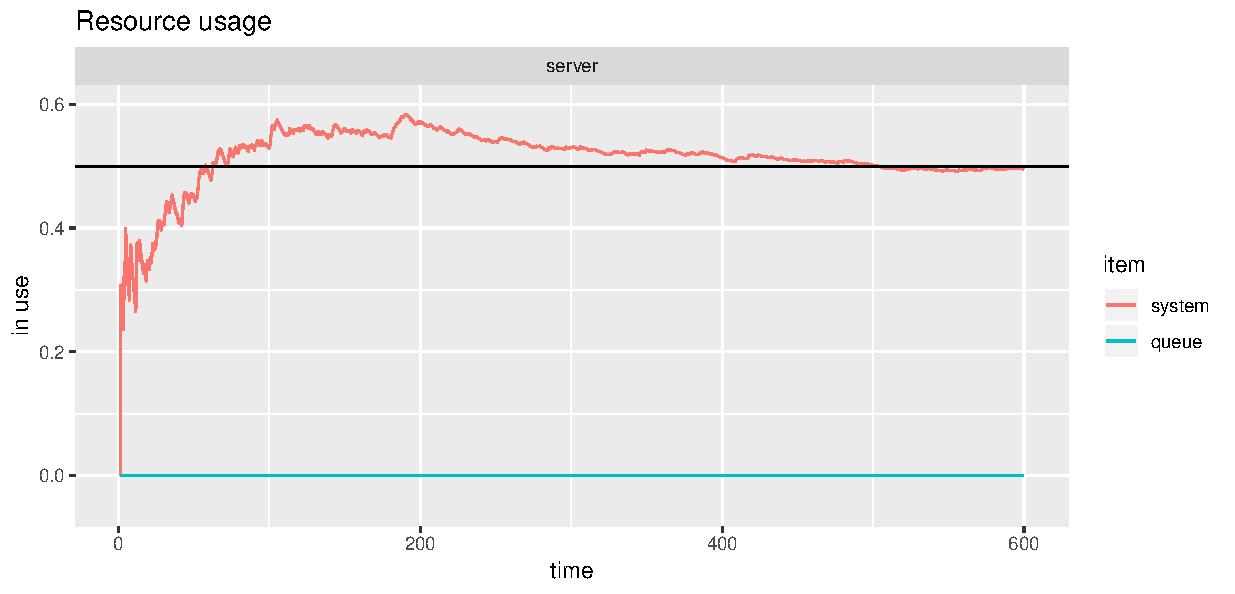
\includegraphics[scale=.75]{figs/Rplot.pdf}
    \caption{Tiempo en el sistema.}
    \label{fig:res}
\end{figure}